\chapter{Esercizi}

\section{Esercizi venerdi 13/03/2026}
\begin{figure}[H]    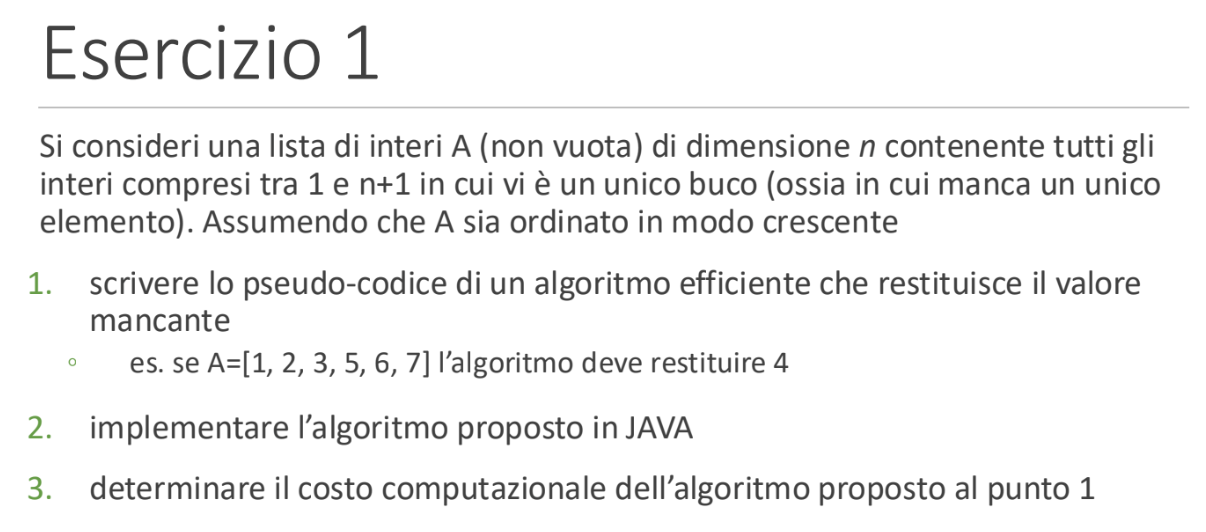
\includegraphics[width=0.75\linewidth]{../images/Screenshot 2026-03-13 alle 10.15.09.png}
    
\end{figure}

\noindent \textbf{1.}\\
\begin{verbatim}
    Trova_buco(A,i,j)
        if(A[i] != i e |A| > 1)
            return i
        if(A[j] = j e |A| > 1)
            return j+1
        if(|A|=1)
            if(A[i] != i)
                return 1
            else return 2
        q = punto medio tra i e j
        if q = A[q]
            Trova_buco(q+1,j)
        else
            Trova_buco(i,q)
\end{verbatim}
\noindent All'inizio mi trovo on i=1 e j=7, nel primo if controllo se c'è il buco nel primo elemento e lo restituisco. Nel secondo if controllo se c'è il buco nell'ultimo elemento.\\
\begin{figure}[H]
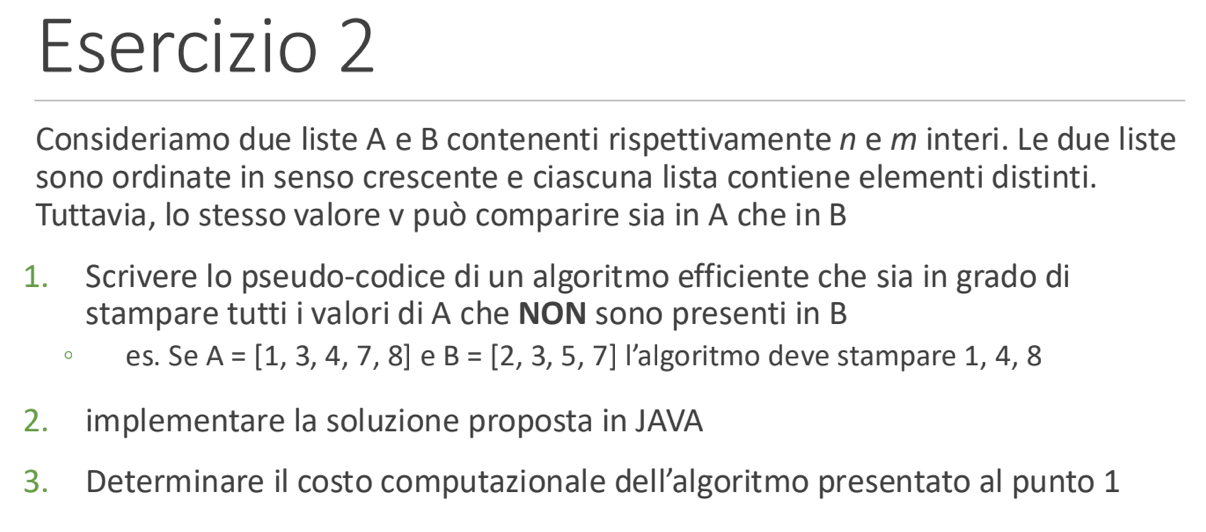
\includegraphics[width=0.75\linewidth]{../images/Screenshot 2026-03-13 alle 10.45.07.png}
    
\end{figure}
\noindent \textbf{1.}
$$A = [1, 3, 4, 7, 8] \text{ con } |A| = n$$
$$B = [2, 3, 5, 7] \text{ con } |B| = m$$
Procedura merge-sort, uso indice $i$ per $A$ e $j$ per $B$:

\begin{verbatim}
    A = [1, 3, 4, 7, 8]
         ^  
         |        
         i
         
    B = [2, 3, 5, 7]
         ^  
         |        
         j
         
\end{verbatim}
\noindent Questo è lo pseudocodice:
\begin{verbatim}
i = 1
j = 1
while (i <= n AND j <= m)
    if(A[i] < B[j])
        stampo(A[i])
        i = i + 1
    else if (A[i] > B[j])
            j = j + 1
        else 
            i = i + 1
            j = j + 1
while(i <= n)
        stampo A[i]
        i = i + 1 
\end{verbatim}
da correggere per quando ci sono i duplicati in $A$\\
Costo algoritmo $n + m$\\
Se non era ordinato comunque aveva un vantaggio prima ordinare le due liste e poi applicare il merge invece di fare la ricerca binaria
\begin{figure}[H]
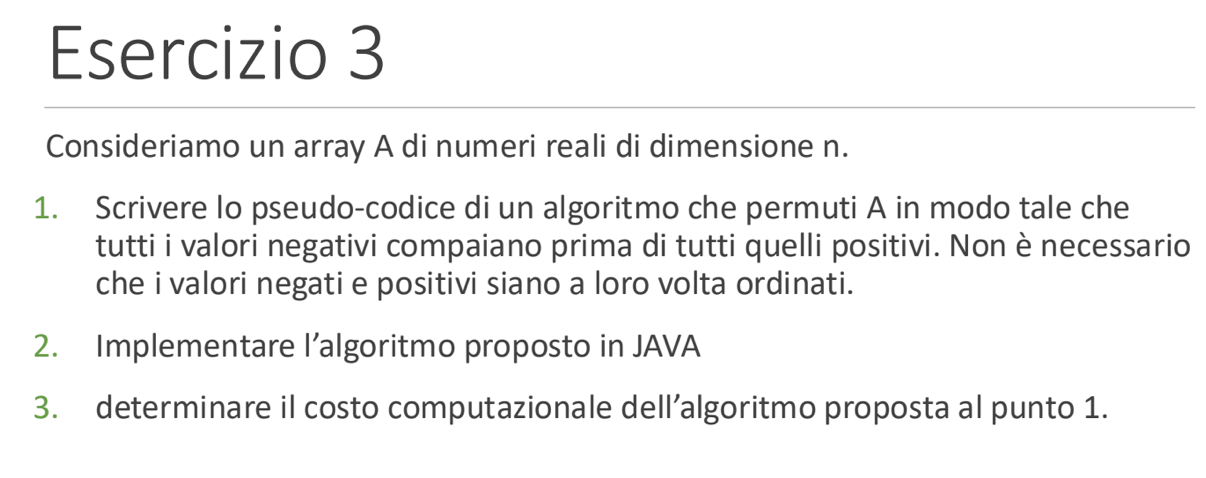
\includegraphics[width=0.75\linewidth]{../images/Screenshot 2026-03-13 alle 11.14.01.png}
    
\end{figure}
\noindent \textbf{1.}\\
In qeusto caso usiamo Quick sort con pivot=0.\\
\begin{verbatim}
    A = [-1, 7, 15, -3, 2, 8, -10]
       ^ ^ 
       | |      
       i j
\end{verbatim}
\begin{verbatim}
    A = [-1, 7, 15, -3, 2, 8, -10]
         ^ 
         |      
        j,i
\end{verbatim}
\begin{verbatim}
    A = [-1, 7, 15, -3, 2, 8, -10]
         ^           ^
         |           |
         i           j
\end{verbatim}
\noindent pseudocodice
\begin{verbatim}
while(j <= |A|)
    if(A[j] < 0)
        swap(A[i+1], A[j])
        i++
    j++
\end{verbatim}


\newpage

\section{Esercizi venerdì 17/04/2026 (Tabelle Hash)}
\begin{figure}[H]
     
    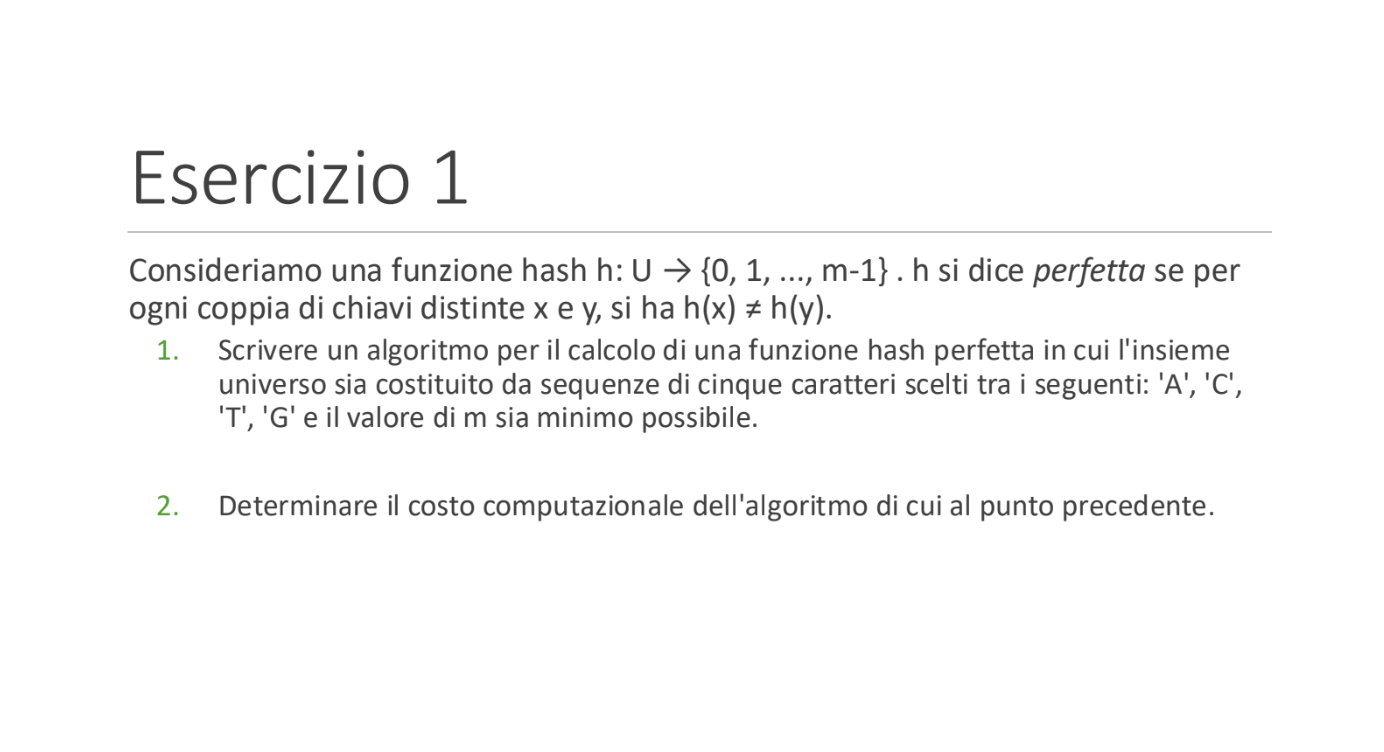
\includegraphics[width=0.7\linewidth]{../images/esercizio1_hash.png}
\end{figure}
Abbiamo che $S$ è:
\[  S = \{ \text{stringhe di lunghezza 5 con i soli caratteri }  
\ 'A', \ 'C', \ 'T', \ 'G' \}  \]
In $S$ ci sono stringhe del tipo: "AAAAA", "AAAAC", "AAACA",..., quindi $|S|$ (cardinalità di $S$)
è calcolata come tutte le permutazioni di 4 caratteri in 5 blocchi, quindi $|S|$ è:
\[  |S| = 4^5 \]
Di conseguenza anche la dimensione della tabella hash è $m = 4^5$.\smallskip\\
Per calcolare la funzione hash perfetta associamo ad ogni carattere un numero da 0 a 4:

    \begin{verbatim}
                                A     C     T     G      
                                |     |     |     |
                                0     1     2     3
\end{verbatim}
L'algoritmo per la funzione hash perfetta è questo, $\forall \ s \in S$:
\begin{enumerate}
    \item converti $s$ in base 4.
    \item converti $s$ da base 4 in base 10.
    \item restituisci la tabella.
\end{enumerate}

\noindent Qual è il costo di questo algoritmo?
\begin{itemize}
    \item il passaggio (1) ha costo costante.
    \item il passaggio (2) ha costo constante.
\end{itemize}
In totale l'algortimo ha costo costante.



\newpage


\begin{figure}[H]
      
    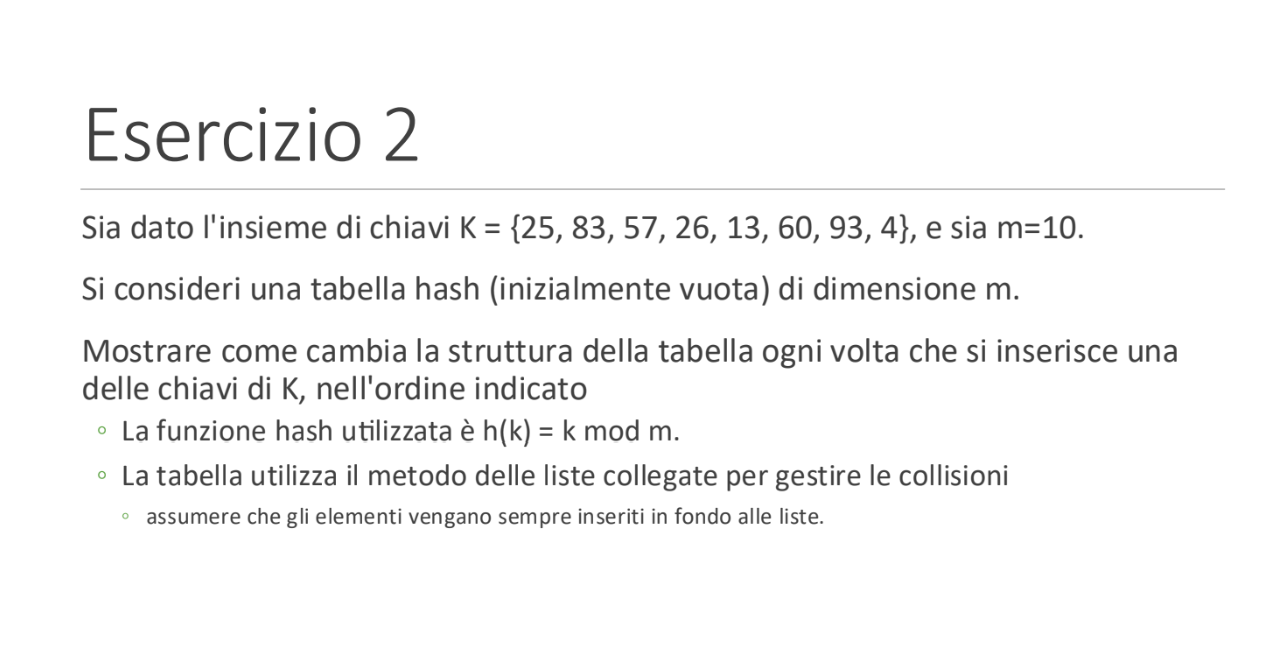
\includegraphics[width=0.8\linewidth]{../images/esercizio2_hash.png}
\end{figure}
\noindent Abbiamo una tabella hash da riempire di dimensioni $m = 10$, e delle chiavi:
\[ K = \{ 25,83,57,26,13,60,93,4  \}  \]
Per gestire le collisioni dobbiamo usare il metodo delle liste collegate, quindi quando
troviamo che in una cella corrispondente ad una chiave c'è già un valore, "agganciamo" a quel valore
il nuovo valore che dobbiamo inserire.\\
La funzione hash è:
\[ h(k) = k \mod m  = \boxed{k \mod 10} \]
\begin{minipage}{0.45\textwidth}
    \begin{itemize}
        \item $h(25) = 25 \mod 10 = \textcolor{red}{5}$
        \item $h(83) = 83 \mod 10 = \textcolor{red}{3}$
        \item $h(57) = 57 \mod 10 = \textcolor{red}{7}$
        \item $h(26) = 26 \mod 10 = \textcolor{red}{6}$
        \item $h(13) = 13 \mod 10 = \textcolor{red}{3}$, collego a $83$
        \item $h(60) = 60 \mod 10 = \textcolor{red}{0}$
        \item $h(93) = 93 \mod 10 = \textcolor{red}{3}$, collego a $13$
        \item $h(4) = 4 \mod 10 = \textcolor{red}{4}$
    \end{itemize}
\end{minipage}
\hfill
$\longrightarrow$
\hfill
\begin{minipage}{0.45\textwidth}
    \begin{figure}[H]
    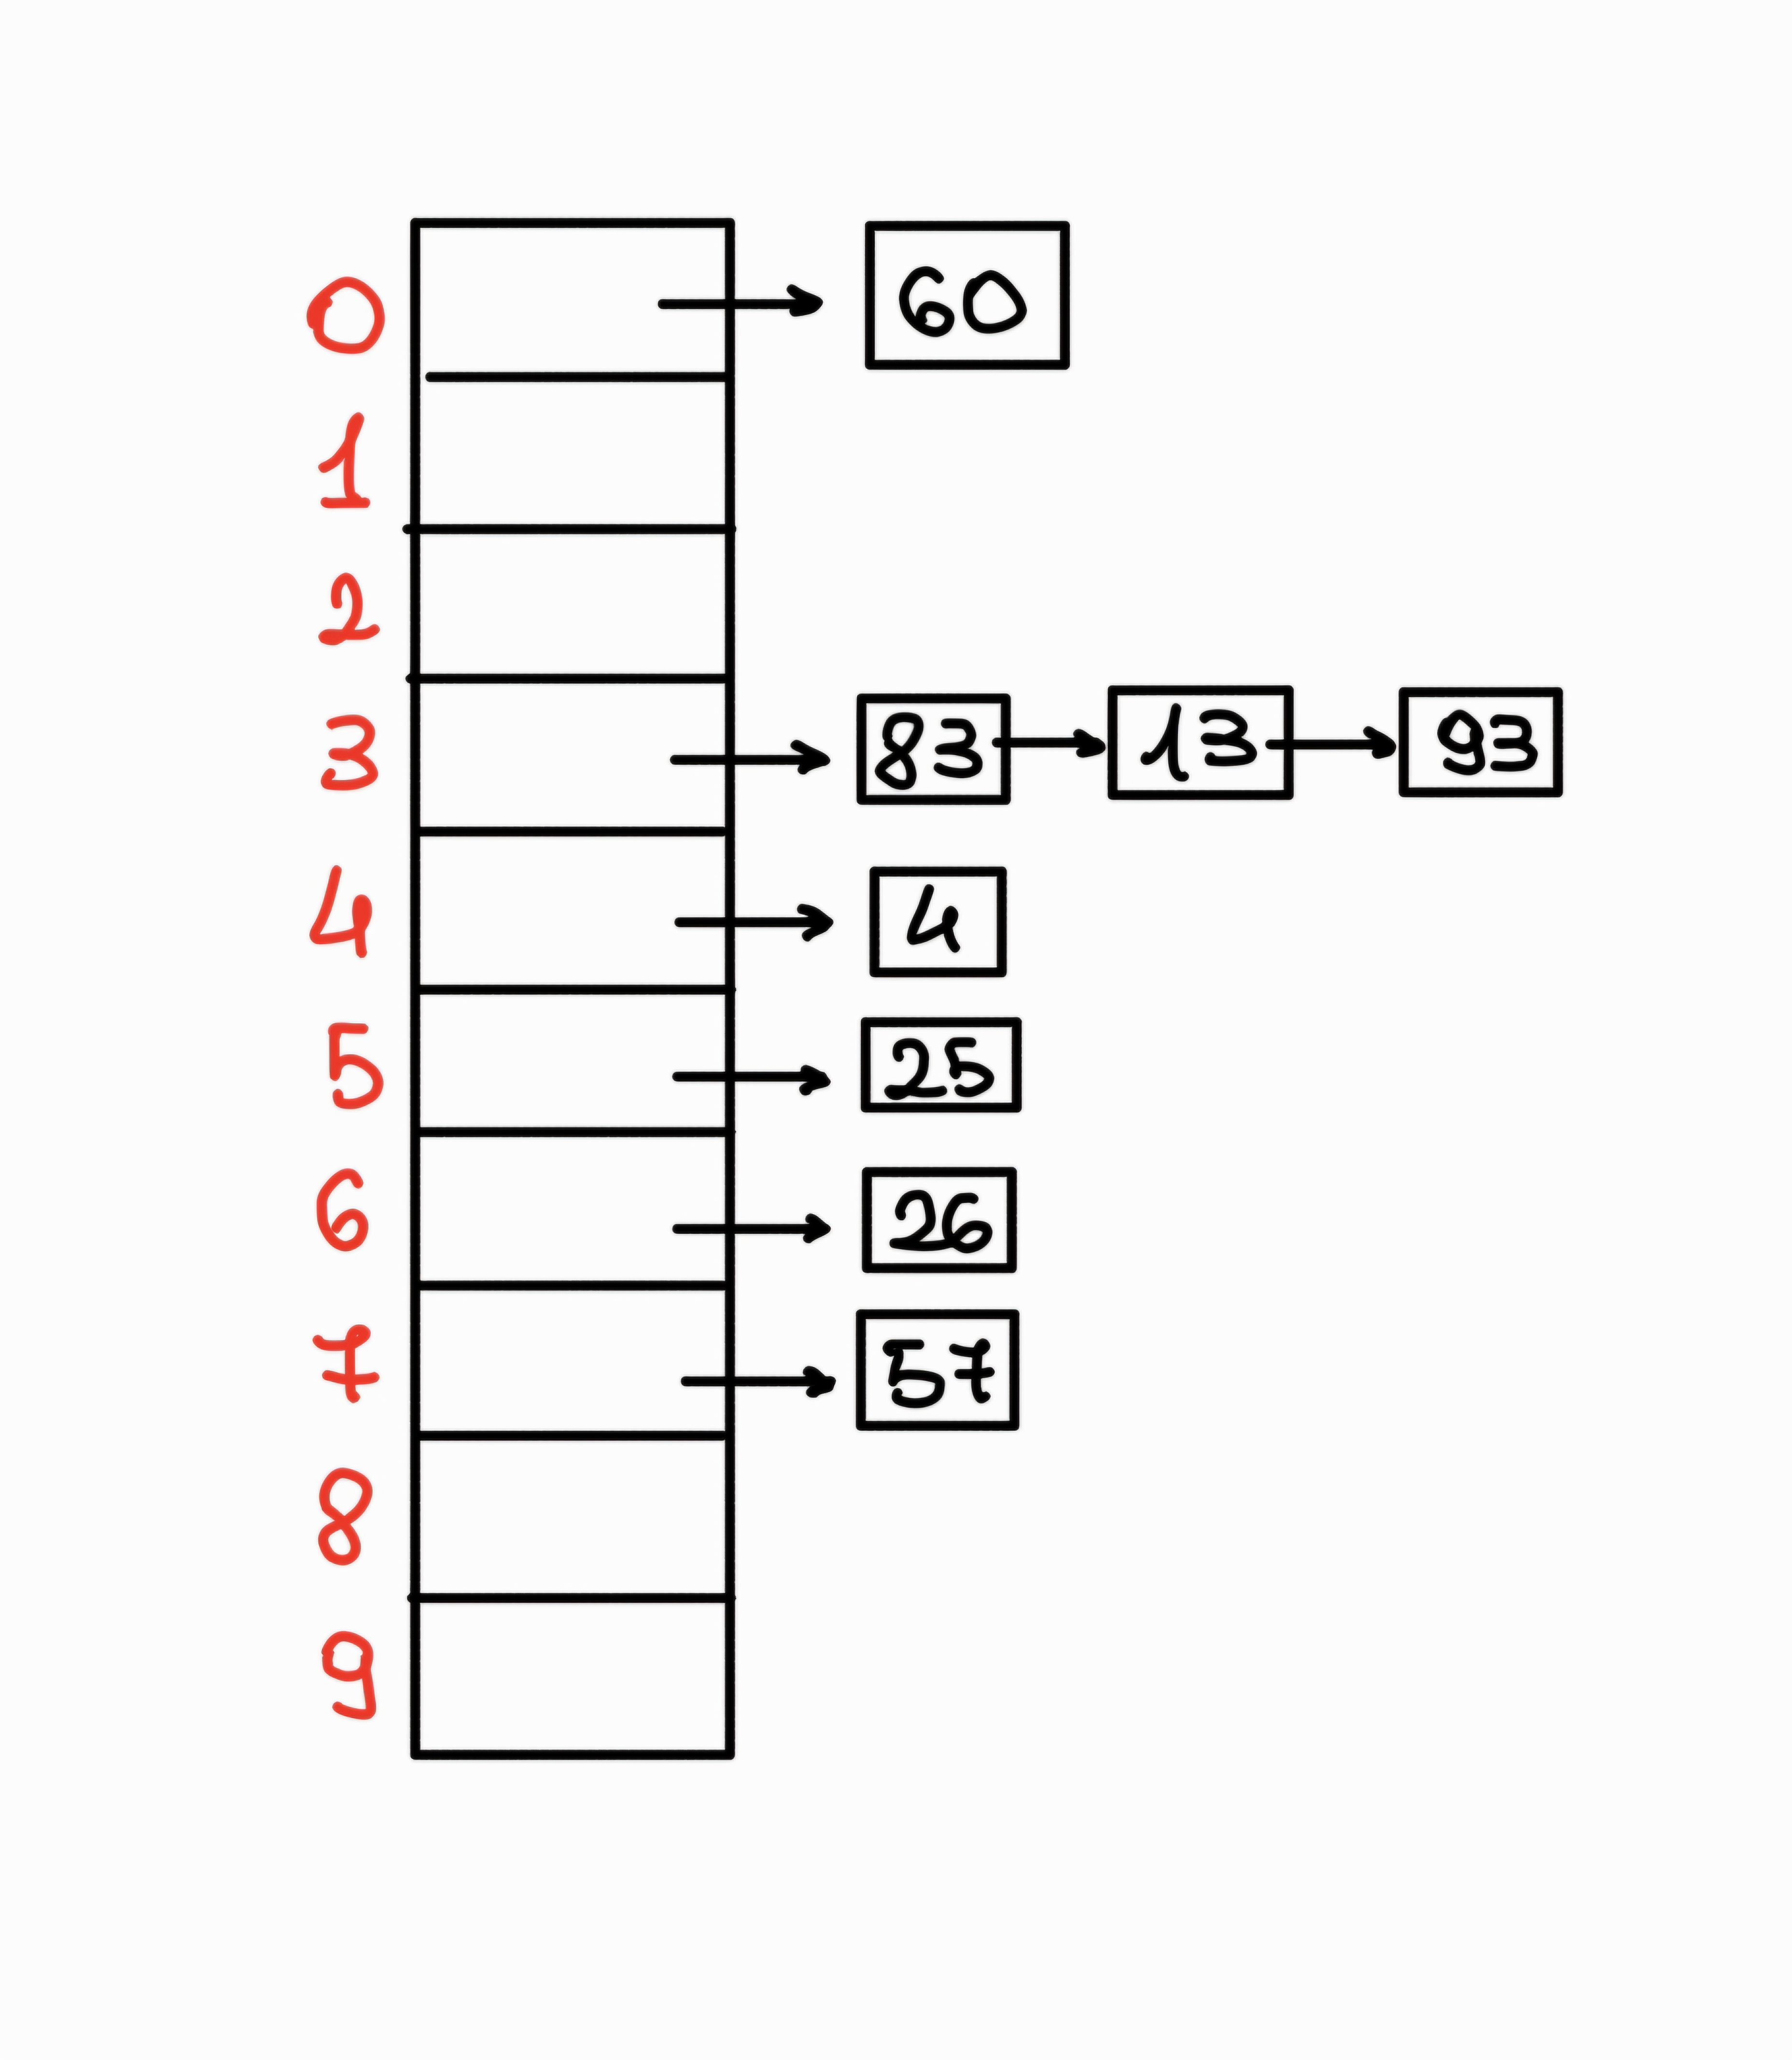
\includegraphics[width=0.8\linewidth]{../images/tab_hash_es2.jpg}
\end{figure}
\end{minipage}





\newpage

\begin{figure}[H]
     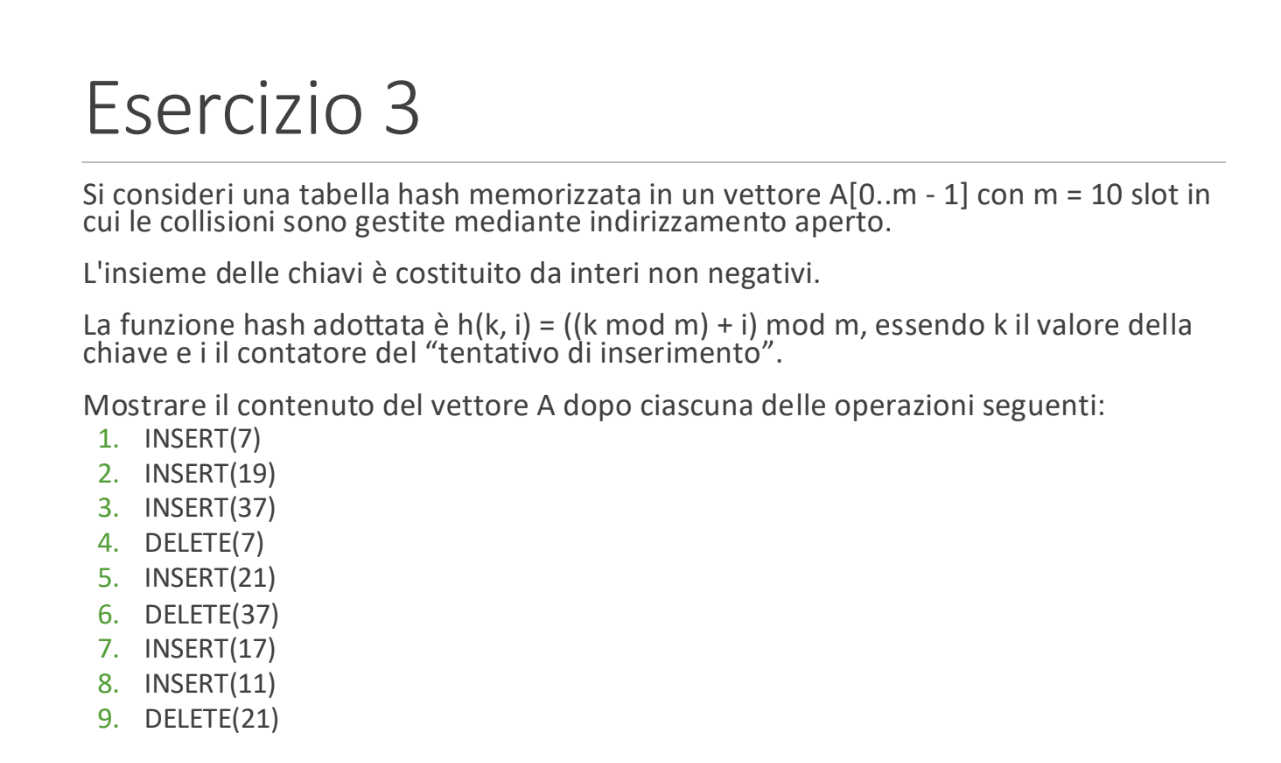
\includegraphics[width=0.8\linewidth]{../images/esercizio3_hash.png}
\end{figure}
La tabella hash ha dimensione $m = 10$, e la funzione di hash è la seguente:
\[ h(k,i) = \left( (k\mod m) + i  \right)  = \boxed{\left( (k\mod 10) + i  \right)} \]
dove:
\begin{itemize}[label=-]
    \item \textbf{k} è la chiave
    \item \textbf{i} è il contatore per i tentativi di inserimento
\end{itemize}
Le collisioni verrano gestiti con indirizzamento aperto, quindi se una cella è già occupata, semplicemente 
il valore non verrà inserito e incrementiamo il contatore $i$, fino a quando non troviamo una cella libera.\medskip\\
\begin{minipage}{0.45\textwidth}
    \begin{itemize}
        \item \texttt{INSERT(7)}: $h(7,0) = 7 \mod 10 + 0 = \textcolor{red}{7}$
        \item \texttt{INSERT(19)}: $h(19,0) = 19 \mod 10 + 0 = \textcolor{red}{9}$
        \item \texttt{INSERT(37)}: $h(37,0) = 37 \mod 10 + 0 = \textcolor{red}{7}$, occupato da 7
        \begin{itemize}
            \item $h(37,1) = 37 \mod 10 + 1 = \textcolor{red}{8}$
        \end{itemize}
        \item \texttt{DELETE(7)}: 7 diventa NULL
        \item \texttt{INSERT(21)}: $h(21,0) = 21 \mod 10 + 0 = \textcolor{red}{1}$
        \item \texttt{DELETE(37)}: 37 diventa NULL
        \item \texttt{INSERT(17)}: $h(17,0) = 17 \mod 10 + 0 = \textcolor{red}{7}$, occupato da NULL
        \begin{itemize}
            \item $h(17,1) = 17 \mod 10 + 1 = \textcolor{red}{8}$, occupato da NULL
            \item $h(17,2) = 17 \mod 10 + 2= \textcolor{red}{9}$, occupato da 19
            \item $h(17,3) = 17 \mod 10 + 3 = \textcolor{red}{0}$
        \end{itemize}
        \item \texttt{INSERT(11)}: $h(11,0) = 11 \mod 10 + 0 = \textcolor{red}{1}$, occupato da 21
        \begin{itemize}
            \item $h(11,1) = 11 \mod 10 + 1 = \textcolor{red}{2}$
        \end{itemize}
        \item \texttt{DELETE(21)}: 21 diventa NULL
    \end{itemize}
\end{minipage}
\hfill
$\longrightarrow$
\hfill
\begin{minipage}{0.45\textwidth}
    \begin{figure}[H]
    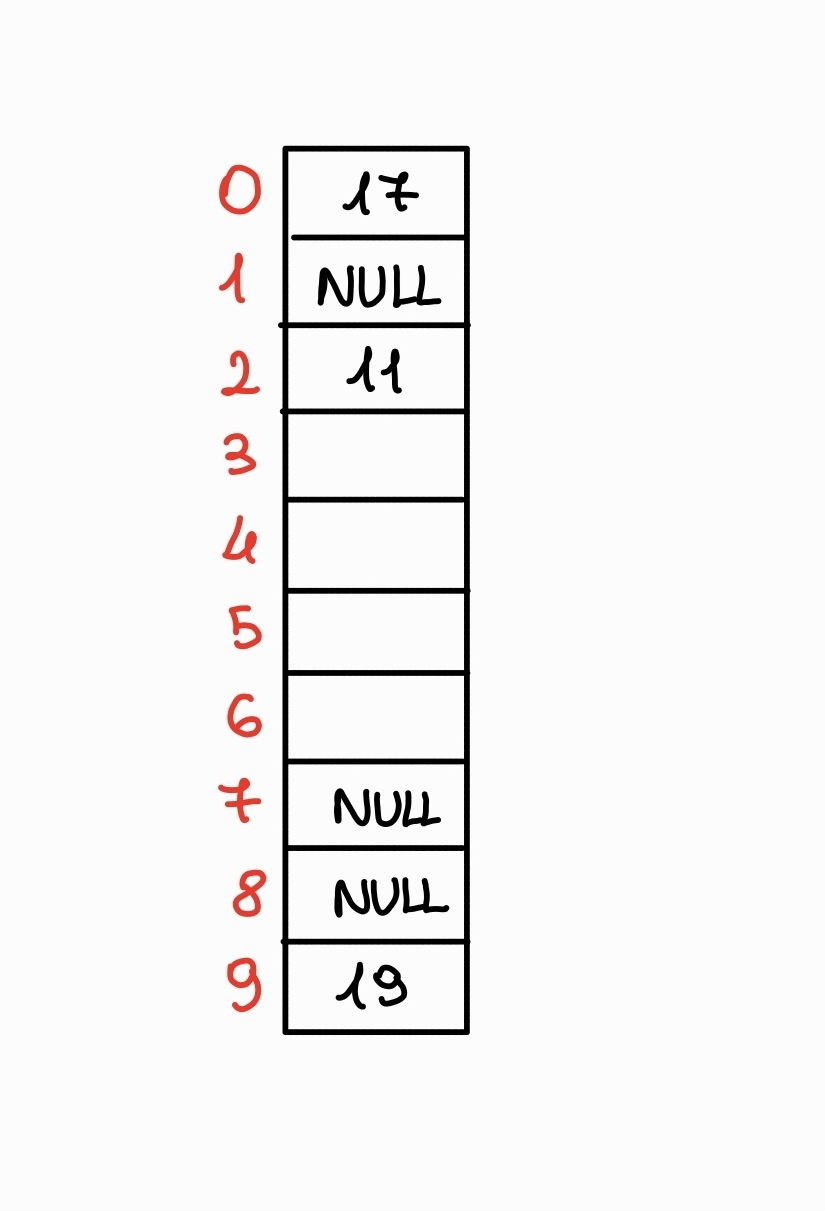
\includegraphics[width=0.8\linewidth]{../images/tab_hash_es3.jpg}
\end{figure}
\end{minipage}


